% The FYP template is designed according to NTU SCSE FYP guidelines on https://www3.ntu.edu.sg/scse/fyp/UsefulInfo/Report%20Guide.pdf.

% Credit
% Original version by Vincent Ribli
% https://www.overleaf.com/latex/templates/ntu-scse-fyp-template/kwdtcbqmjctk

% Revised by Prof Loy Chen Change
% 23 Aug 2024 - Replace SCSE with CCDS

\documentclass[pdftex, 12pt, a4paper]{report}
\usepackage{newtxtext, newtxmath}
\usepackage[top=3cm, bottom=3cm, left=3.5cm, right=3cm]{geometry}
\usepackage[hidelinks]{hyperref}
\usepackage[pdftex]{graphicx}
\usepackage{booktabs}
\usepackage{setspace}
\usepackage{titlesec}
\usepackage{tocloft}
\usepackage{parskip}
\usepackage{amsmath}
\usepackage{amsfonts}
\usepackage[sorting=none]{biblatex}
\usepackage{graphicx}
\usepackage{longtable}
\usepackage{array}
\usepackage{float}

\addbibresource{bib.bib}
\setstretch{1.5}
\setlength{\cftfigindent}{0pt}
\setlength{\cfttabindent}{0pt}
\renewcommand{\cftdotsep}{1}

% change the following
\title{\uppercase{{TextLens - A translation App Integrated with Scene Text Editing}}}
\newcommand\fypcode{CCDS25-0235}
\author{Goh Yew Kiang}
\date{2026}
\newcommand\degree{Bachelor of Computing in Computer Science}

\usepackage{biblatex}
\addbibresource{references.bib}

\begin{document}
\input{cover.tex}
\input{title.tex}

\setcounter{page}{1}
\pagenumbering{roman}

\chapter*{Abstract}
\addcontentsline{toc}{chapter}{Abstract}

Real-time camera translation has become increasingly common through applications such as Apple Translate and Google Lens. However, the internal design and implementation details of these systems are largely proprietary, making it difficult to understand how their translation pipelines function or how similar capabilities can be reproduced in an offline environment. This project presents \textit{TextLens}, a mobile application designed to perform real-time scene text translation directly on an Android device without requiring continuous internet connectivity.

TextLens integrates computer vision and natural language processing into an on-device processing pipeline that captures camera frames, detects and recognizes scene text, translates the detected content, and renders the translated text back into the original image. The system uses ML Kit on-device optical character recognition (OCR) and neural machine translation models, allowing the application to function fully offline once language models are installed. To improve visual quality, a scene text replacement module removes original text regions using image inpainting and redraws translated text, tracking the text and inpainting in real-time.

Evaluation results demonstrate strong performance, achieving an OCR character error rate of 5.9\%, detection precision of 92.1\%, detection recall of 86.8\%, and a translation quality score of 4.2/5. These results show that practical real-time multilingual scene translation can be achieved using an entirely on-device mobile pipeline.

\chapter*{Acknowledgments}
\addcontentsline{toc}{chapter}{Acknowledgments}

I would like to express my sincere gratitude to my supervisor, Dr Loke Yuan Ren, for his guidance, support, and valuable feedback throughout the course of this project. His insights and suggestions were instrumental in shaping the direction of this work and helped me refine both the technical implementation and the research aspects of the project.

I would also like to thank the Nanyang Technological University, College of Computing and Data Science, for providing the resources and learning environment that made this project possible.

Finally, I would like to express my appreciation to my friends and family for their encouragement and support during the development of this project.




\pagebreak
\addcontentsline{toc}{chapter}{Contents}
\tableofcontents

\pagebreak
\addcontentsline{toc}{chapter}{List of Tables}
\listoftables

\pagebreak
\addcontentsline{toc}{chapter}{List of Figures}
\listoffigures

\cleardoublepage
\pagenumbering{arabic}

\chapter{Introduction}

\section{Background}

With the increasing globalization of communication, mobile applications that provide instant translation have become very important for travelers, students, and professionals. Google Translate alone has surpassed one billion installations worldwide \cite{pitman2021googletranslate}. Among the various translation technologies available today, real-time camera-based translation has emerged as a particularly useful solution. By pointing a smartphone camera at text in the physical environment—such as signs, menus, and documents—users can instantly view translated content overlaid on the captured scene. These systems typically combine optical character recognition (OCR) to detect and extract text from images with machine translation (MT) to convert the recognized text into a target language.

Despite significant advances in OCR and neural machine translation, real-time camera-based translation remains a challenging problem \cite{ocr_issues}. Text appearing in natural scenes often exhibits large variations in lighting conditions, font styles, orientations, and background complexity, which can negatively affect the accuracy of text detection and recognition. In addition, real-time camera input introduces motion blur and frame instability, which may lead to repeated OCR processing and unstable or flickering translated overlays.

Another important challenge lies in the visual presentation of translated text. Many existing systems render translated text directly over the original text without preserving visual properties such as colour, scale, or orientation. This may result in overlays that appear inconsistent with the surrounding scene and reduce readability. Furthermore, many commercial camera translation systems rely heavily on cloud-based processing, which introduces latency, raises privacy concerns, and limits usability in environments with poor or no internet connectivity. These limitations highlight the need for mobile translation systems that can operate efficiently, accurately without the need of a stable internet connection.

\section{Motivation}

In an increasingly globalized world, the ability to understand foreign-language text has become important in both professional and everyday contexts. However, language barriers continue to hinder communication and accessibility, particularly when users encounter unfamiliar languages in physical environments. Situations such as travelling abroad, reading product labels, navigating public transportation systems, or understanding restaurant menus can become difficult when translation tools are unavailable or unreliable.

Many existing translation applications rely on cloud-based processing, which requires continuous internet connectivity. In real-world scenarios, however, reliable internet access may not always be available. Users travelling in rural areas, underground transport systems, or foreign countries with limited connectivity may find online translation tools difficult to use.

This project is motivated by the need for a mobile translation system that can function reliably without continuous internet access. By performing text recognition and translation directly on the mobile device, the system can provide real-time translation capabilities even in offline environments. Such a solution can improve accessibility, support cross-cultural communication, and provide a more convenient user experience when interacting with multilingual environments.

\section{Project Objectives}

The main objective of this project is to develop an offline, real-time mobile scene text translation application for Android that can detect, recognize, translate, and replace text in natural scenes without requiring continuous internet connectivity. The project aims to demonstrate how computer vision, optical character recognition, and mobile software engineering can be integrated into a practical end-user application.

The specific objectives of this project are as follows:

\begin{enumerate}
    \item To design and implement a mobile translation system that operates without Wi-Fi or constant network connectivity by utilizing on-device text recognition and translation models.

    \item To develop a complete end-to-end processing pipeline that captures camera frames, performs text detection and recognition, translates the detected text, and renders the translated results back onto the scene.

    \item To integrate multiple computer vision components—including frame acquisition, preprocessing, OCR triggering, text tracking, image inpainting, translated text rendering—into and tracking a unified application.

    \item To implement the solution as a fully functional Android application using Android Studio, demonstrating a deployable mobile software system rather than a conceptual prototype.

    \item To design a user-friendly interface that allows users to interact easily with the application through features such as language selection, live camera preview, and freeze-frame viewing.
\end{enumerate}

\section{Project Scope}

The scope of this project covers the design, implementation, integration, and evaluation of an Android-based mobile application for offline scene text translation. The project focuses on building a working prototype that demonstrates the complete translation workflow in real time and highlights the integration of several computer vision modules within a mobile environment.

The project scope includes the following components:

\begin{enumerate}

    \item \textbf{Offline mobile deployment}

    The system is designed specifically for Android devices and performs the main processing tasks directly on the device. The application is intended to operate without continuous reliance on cloud services or internet connectivity during normal usage.

    \item \textbf{Real-time camera-based text translation}

    The application processes live camera input and performs translation on text appearing within the captured scene. The workflow includes frame acquisition, text recognition, translation, and visual rendering of translated text in near real time.

    \item \textbf{End-to-end computer vision pipeline}

    The project implements and integrates multiple processing modules, including:
    
    \begin{itemize}
        \item camera frame acquisition
        \item frame preprocessing
        \item OCR triggering under stable frame conditions
        \item multilingual text recognition
        \item text region tracking between OCR updates
        \item image inpainting for removal of original text
        \item translated text rendering within the scene
    \end{itemize}

    \item \textbf{Tracking System}
      The project includes a motion-aware text tracking module that maintains the position of detected text regions between OCR updates. After an OCR pass detects text, the system tracks the text boxes across subsequent camera frames so that translated overlays remain aligned even when the device or scene moves slightly.    

    \item \textbf{Mobile user interface design}

    The project includes the design of a usable mobile interface, including features such as live camera preview, language selection controls, translated text display, and freeze-frame interaction to improve readability.

    \item \textbf{Application integration and packaging}

    The system integrates all components into a complete Android Studio project and packages them into a functional mobile application prototype for demonstration and evaluation.

\end{enumerate}

This project does not include large-scale cloud deployment, server-based translation services during runtime, or support for every possible language and device type. Instead, the focus is on developing a practical offline prototype that demonstrates the core concept of real-time multilingual scene text translation on Android devices.

\section{Contributions}

This project contributes the design and implementation of an offline, real-time mobile scene text translation system on Android. The main contributions of this work are summarized as follows:

\begin{enumerate}

\item \textbf{Offline real-time translation system}

The project demonstrates a translation application that does not depend on continuous internet connectivity. By performing text recognition and translation directly on the device, the system remains usable in environments with limited or no network access.

\item \textbf{End-to-end mobile translation pipeline}

A complete processing pipeline is implemented, starting from live camera capture and progressing through text detection, recognition, translation, and visual rendering of translated text within the scene.

\item \textbf{Integration of multiple computer vision components}

The project integrates several computer vision and image processing modules—including frame acquisition, OCR detection, text region tracking, image inpainting, and text rendering—into a unified system suitable for mobile deployment.

\item \textbf{Tracking system}

The project contributes a tracking mechanism that preserves detected text regions between OCR updates, allowing translated text to remain aligned with the scene while reducing the need for repeated full recognition. This improves efficiency and supports smoother real-time performance on mobile hardware.   

\item \textbf{Deployment as a functional Android application}

The project demonstrates a working Android application that integrates computer vision, natural language processing, and mobile software engineering into a deployable system.

\item \textbf{Practical demonstration of on-device AI}

The project illustrates how computer vision and natural language processing models can be deployed directly on mobile devices to perform complex tasks without relying on cloud-based computation.

\end{enumerate}
\chapter{Literature Review}

\section{Related works}

\subsection{Google Translate}

Google Translate is a widely used real-time translation application that supports multiple input modalities, including text, voice, handwriting, and camera images. The system produces translated outputs in both text and speech formats, and in the case of camera input, translated text can be displayed directly over the captured image.

The translation component of Google Translate is based on Google's Neural Machine Translation (GNMT) system. GNMT employs a deep encoder–decoder architecture built using recurrent neural networks (RNNs) combined with attention mechanisms. This architecture enables the system to model long-range dependencies in sentences, capture complex grammatical structures across different languages, and produce more accurate translations. In later developments, Google incorporated transformer-based architectures to improve translation speed and efficiency.

The main components of the GNMT architecture include:

\begin{itemize}
    \item \textbf{Encoder–Decoder RNNs:} The encoder converts input words into continuous vector representations, while the decoder generates the translated sequence based on these representations.

    \item \textbf{Deep Neural Layers:} GNMT uses multiple stacked RNN layers (up to eight layers) to improve the model's ability to capture complex linguistic patterns and contextual relationships.

    \item \textbf{Attention Mechanism:} The attention mechanism connects the encoder and decoder, allowing the model to focus on relevant parts of the input sentence during translation and helping to mitigate the short-memory limitations of traditional RNN architectures.
\end{itemize}

 It integrates with OCR (for camera input), ASR (speech recognition), and TTS (speech synthesis), making Google Translate multimodal.

\begin{figure}[h]
    \centering
    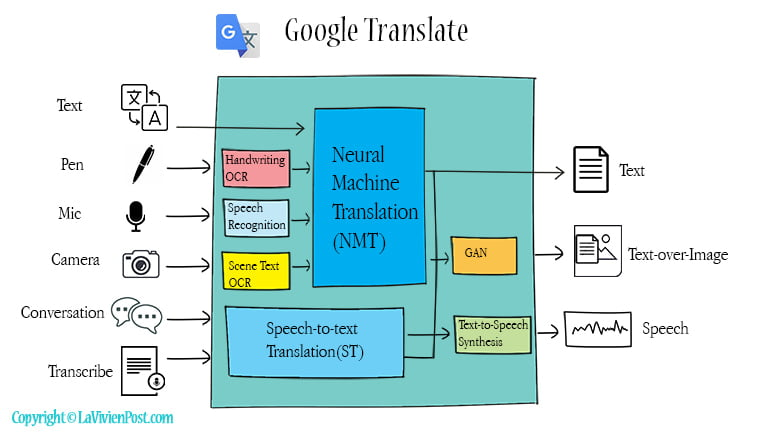
\includegraphics[width=\linewidth]{fig/google-translate.jpg}
    \caption{Architecture overview of Google Neural Machine Translation \cite{vivien2022gnmt}.}
    \label{fig:gnmt}
\end{figure}

\section{Current Research on Individual Components}

\subsection{OCR in Natural Scenes}

Optical Character Recognition (OCR) is widely used to convert printed or handwritten text into a digital form, enabling further processing such as search, editing, or translation \cite{liu2020scenetext}. In natural scene text recognition, the OCR task is typically divided into two stages: text detection and text recognition. The detection stage identifies regions of an image that contain text, while the recognition stage converts the detected text regions into character sequences.

Traditional OCR systems perform well when applied to structured documents with clean backgrounds and consistent fonts. However, scene text recognition presents additional challenges due to variations in lighting conditions, background complexity, perspective distortion, and font diversity \cite{szankin2025seeing}. To address these challenges, modern approaches often rely on deep learning-based models trained on large datasets of natural images.

Recent models such as Ocean-OCR improve robustness by increasing training data scale and model complexity, allowing the system to better handle noisy environments and diverse text styles \cite{chen2025oceanocr}. However, these large models typically require substantial computational resources and introduce higher inference latency. Such approaches are therefore less suitable for real-time mobile applications where computational efficiency is a critical constraint. As a result, lightweight OCR systems that prioritize speed and on-device inference are often used in mobile translation applications, even if this may slightly reduce recognition accuracy in challenging conditions \cite{bagal_2022image_translation}.

\subsection{Language Detection Techniques}

Language detection refers to the process of automatically identifying the language of a given text segment \cite{lui2014automatic}. This capability is important in multilingual translation systems because it allows the system to determine the source language before performing translation.

Two commonly used approaches for language detection are statistical n-gram methods and neural network–based approaches. N-gram methods analyze short character sequences within a text and estimate the probability that the text belongs to a particular language. These methods are computationally efficient and work well for short text segments, making them suitable for mobile applications.

Deep learning approaches, on the other hand, use neural networks to model more complex linguistic patterns and typically achieve higher accuracy \cite{gothe2020language}. However, such models often require greater computational resources and may introduce additional latency during inference. In mobile environments where computational efficiency is important, lightweight detection methods are often preferred.

\subsection{Machine Translation}

Machine translation (MT) is a fundamental task in natural language processing that aims to automatically convert text from one language to another \cite{tsujii1986future}. Early machine translation systems relied on rule-based or statistical approaches, but recent advances have been driven by neural machine translation (NMT).

Neural machine translation models typically employ encoder–decoder architectures that map input sentences into continuous vector representations and generate translated outputs based on these representations. The introduction of attention mechanisms further improved translation performance by allowing the model to focus on relevant parts of the input sentence during decoding.

More recently, transformer-based architectures have become the dominant approach for machine translation, offering improved scalability and parallelization compared to earlier recurrent neural network models \cite{kocmi2022findings}. These advances have significantly improved translation quality and enabled practical applications such as real-time multilingual translation systems.

For mobile translation applications, lightweight on-device translation models are commonly used to balance translation quality with computational efficiency. These models allow translation to be performed locally on the device without requiring continuous network connectivity.

\subsection{Scene Text Editing and Replacement}

Scene text editing refers to the task of modifying text that appears within natural images while preserving the surrounding visual context \cite{wu2019editing}. This problem lies at the intersection of computer vision, image synthesis, and text rendering. The objective is to replace the original text in an image with new content while maintaining consistency with the background, spatial layout, and visual appearance of the scene.

Early approaches to scene text editing often relied on generative adversarial networks (GANs) to jointly model background reconstruction and text generation \cite{wu2019editing}. These methods attempted to generate new text directly within the image while maintaining realistic visual integration with the surrounding scene.

More recent work has explored improved techniques for preserving text structure, font style, and alignment. For example, recognition-aware editing methods incorporate text recognition information to ensure semantic consistency between the generated text and the intended content \cite{fang2025rsste}. Other approaches such as the FASTER framework focus on preserving font appearance and spatial alignment while replacing text content \cite{das2025faster}.

Although these advanced models produce visually convincing results, many of them are computationally expensive and difficult to deploy in real-time mobile applications. For practical mobile systems, simpler techniques such as image inpainting combined with text re-rendering are often used to remove the original text region and insert translated text in a visually coherent manner.
\chapter{Architecture and Technologies}

This chapter explains the overall architecture of \textit{TextLens} and the main technologies used to develop it. It describes how the system is divided into several functional layers and discusses the frameworks, libraries, and tools that were chosen to support offline, real-time scene text translation on Android devices.

\section{TextLens Architecture}

\textit{TextLens} is designed as an \textbf{offline mobile application} that performs scene text detection, recognition, translation, and rendering directly on the device itself. To support this workflow, the system is organised into three main layers, namely the UI layer, the application control layer, and the on-device processing layer. This layered structure makes the application more modular, easier to maintain, and also easier to test during development.

\begin{itemize}
    \item \textbf{UI Layer:}  
    The UI layer is the part of the system that the user interacts with. It is responsible for showing the live camera preview, allowing the user to choose the source and target languages, supporting freeze-frame mode, and displaying the translated text in a way that is easy to read.

    \item \textbf{Application Control Layer:}  
    The application control layer manages the main workflow of the system. It coordinates the camera input, decides when OCR should be triggered, keeps track of frame and detection states, handles communication between the different modules, and ensures that the UI and processing components work properly together.

    \item \textbf{On-Device Processing Layer:}  
    The on-device processing layer performs the main computer vision and language processing tasks. These include camera frame acquisition, image preprocessing, text recognition, language translation, text region tracking, and scene text replacement. Since all of these operations are carried out locally on the device, the application is able to continue functioning even when there is no continuous internet connection.
\end{itemize}

\begin{figure}[H]
    \centering
    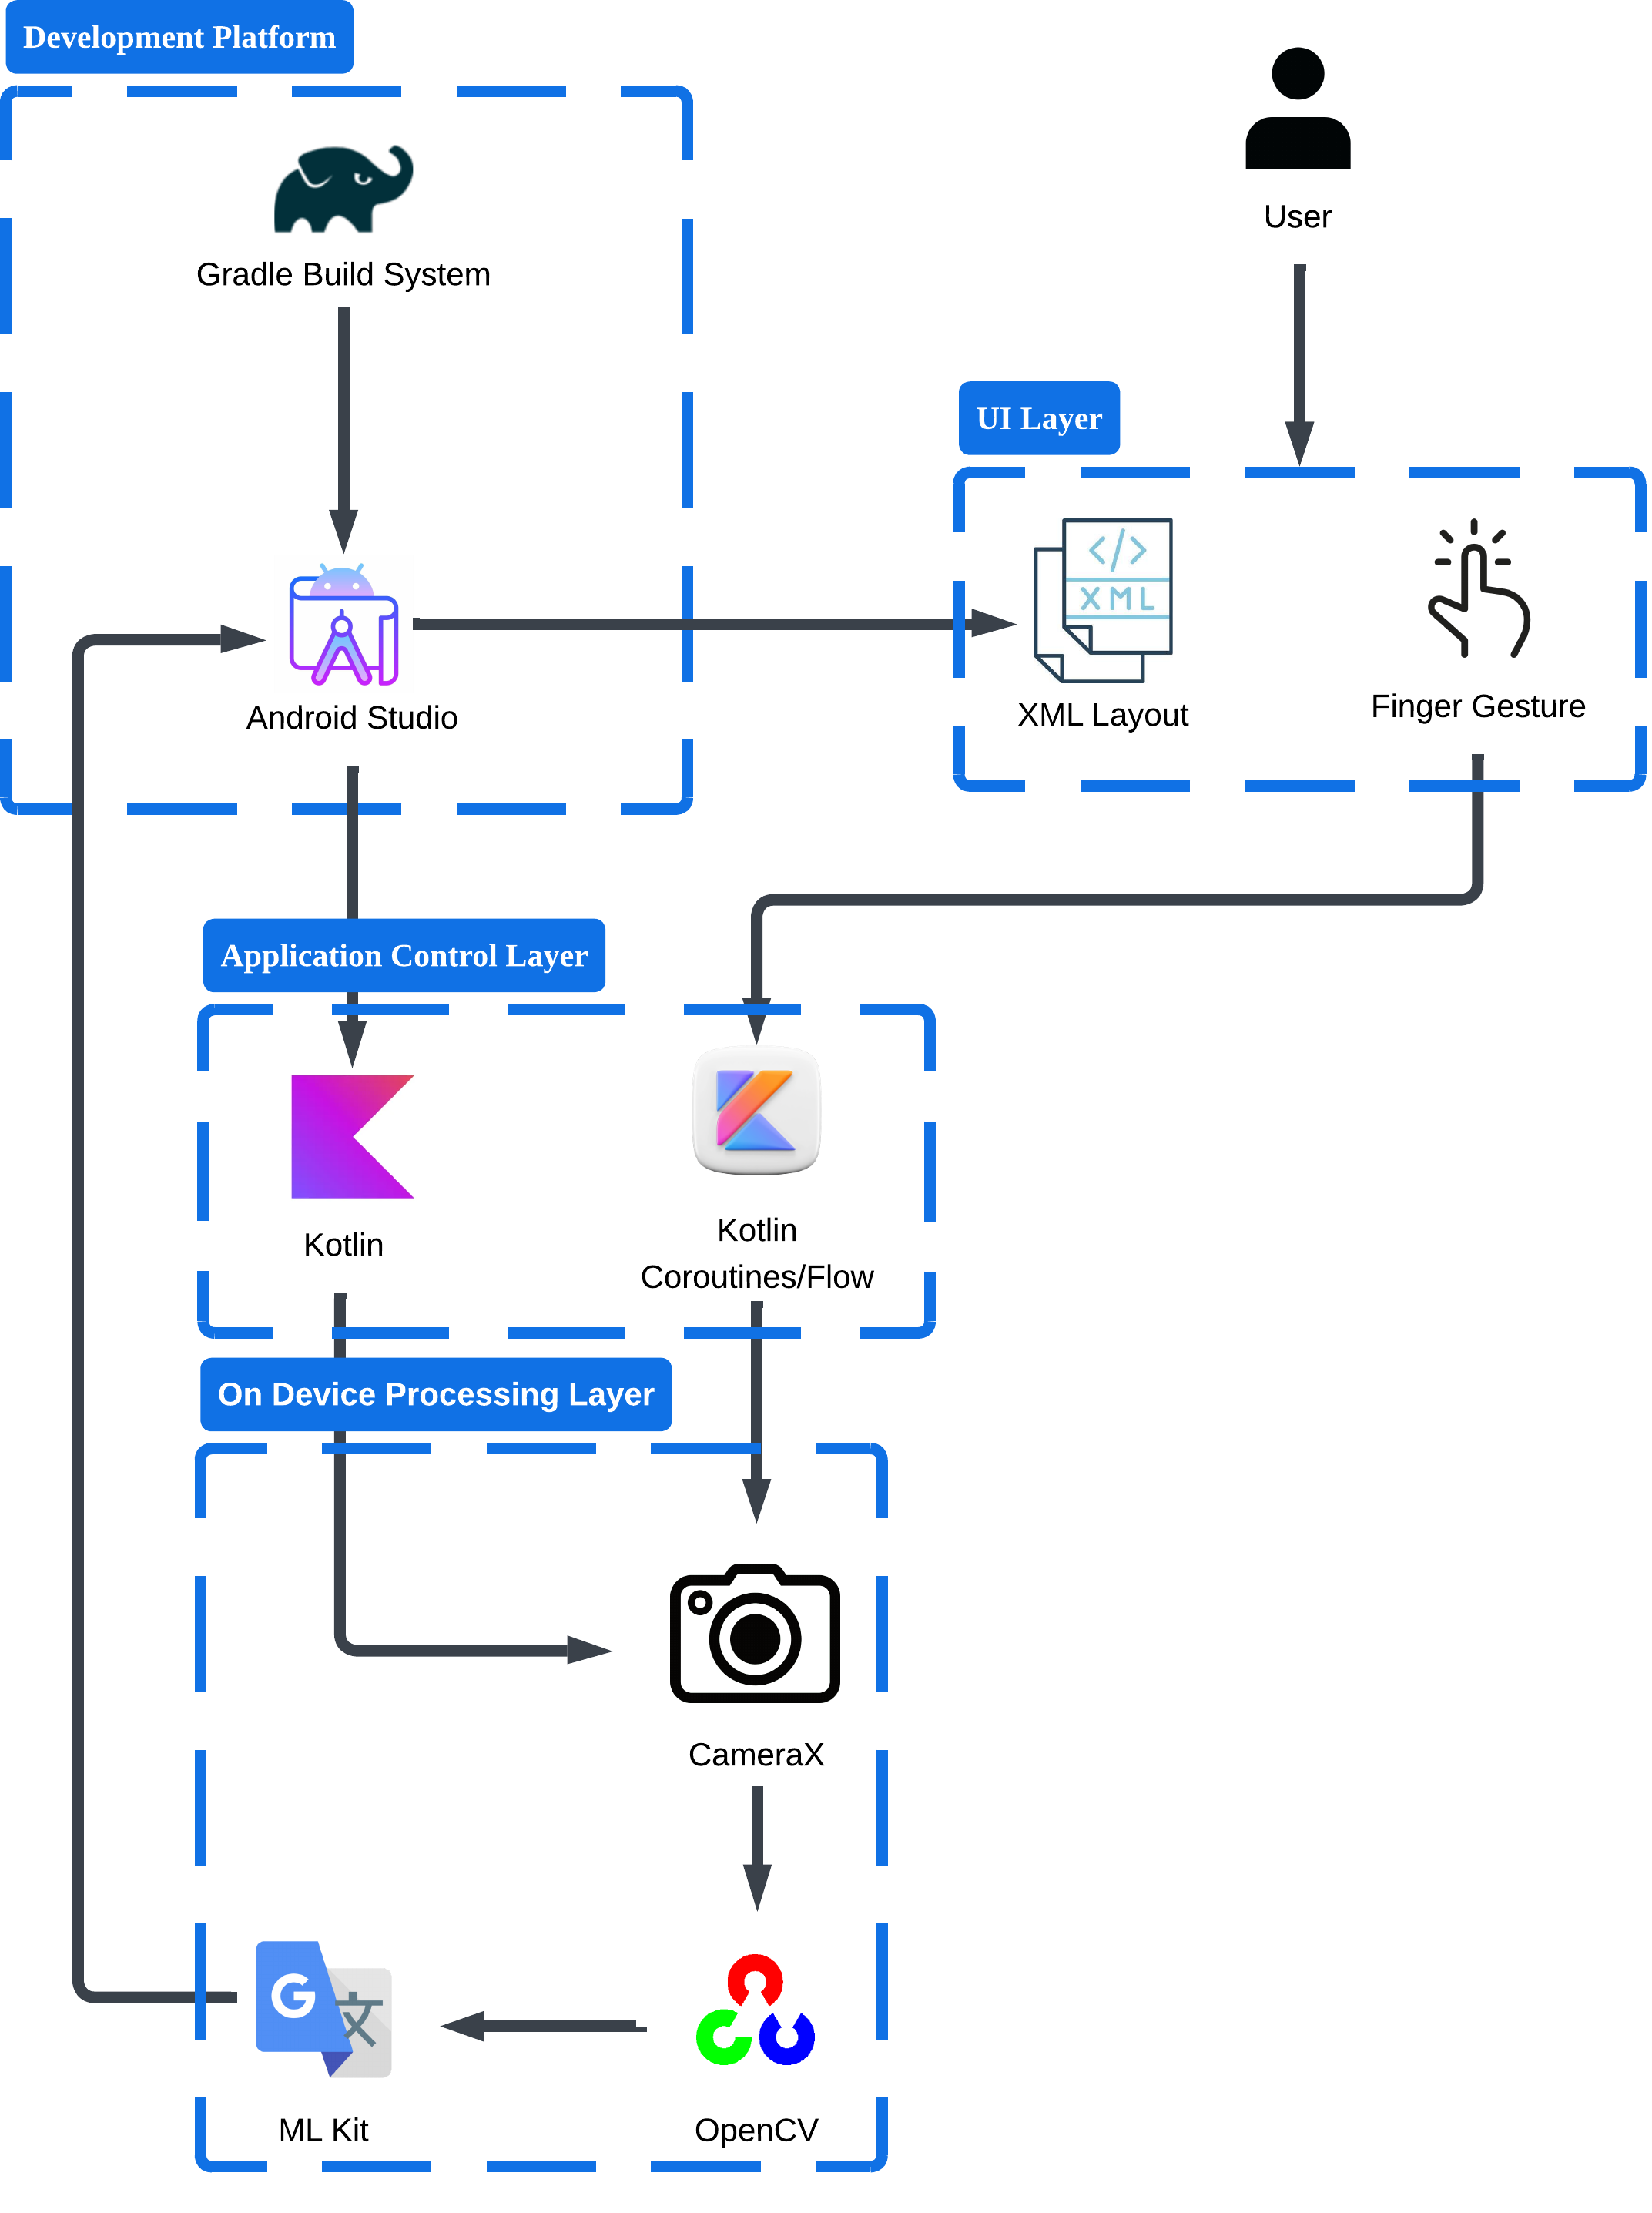
\includegraphics[width=\linewidth]{fig/overview_architecture.png}
    \caption{TextLens architecture overview}
    \label{fig:textlens_architecture}
\end{figure}

\section{Technologies Used}

This section describes the main technologies used in the implementation of TextLens and the rationale for their selection.

\subsection{Frontend and Application Framework}

\subsubsection{Kotlin}
Kotlin is the primary programming language used to develop TextLens. It is officially supported for Android development and provides a concise syntax, strong type safety, and good interoperability with Java-based Android libraries. Its language features also help improve code readability and maintainability.

\subsubsection{XML and Android View System}
The user interface is built using XML layout files together with the Android View system. This approach separates interface design from application logic, making it easier to manage the layout structure, update UI components, and maintain the overall application.

\subsubsection{Android Studio}
Android Studio is used as the main development environment for the project. It provides integrated tools for coding, debugging, dependency management, device emulation, and application packaging, making it suitable for building and testing a full Android application.

\subsubsection{CameraX}
CameraX is used for camera integration and live frame acquisition. It provides a lifecycle-aware API that simplifies camera development and ensures more consistent behaviour across different Android devices. In TextLens, CameraX is used to capture frames for real-time text recognition and translation.

\subsubsection{Kotlin Coroutines and Flow}
Kotlin Coroutines and Flow are used to handle asynchronous and reactive operations in the application. They allow long-running tasks such as OCR, translation, and image processing to run without blocking the UI thread. This helps maintain responsiveness and supports smoother real-time performance.

\subsection{Computer Vision and Language Processing}

\subsubsection{OpenCV}
OpenCV is used for image processing and low-level computer vision operations. In TextLens, it supports tasks such as frame conversion, preprocessing, region handling, inpainting, and image manipulation required for scene text replacement. OpenCV is particularly useful because it provides direct control over pixel-level operations.

\subsubsection{ML Kit Optical Character Recognition (OCR)}
ML Kit's on-device OCR is used to detect and recognize text from camera frames. It provides recognized text together with bounding boxes, which are important for locating text regions in the scene. Since the OCR runs on-device, it supports lower latency and better privacy while allowing the application to operate offline.

\subsubsection{ML Kit Neural Machine Translation}
ML Kit's on-device translation is used to translate recognized text into the user-selected target language. This enables multilingual translation without requiring continuous internet access. The use of on-device translation is an important design choice because it supports the project's objective of offline real-time usability.

\subsubsection{Text Region Tracking}
Text region tracking is used to maintain the position of detected text between OCR updates. This improves the continuity of the displayed translation and reduces the need to run OCR on every frame. Tracking contributes to a smoother and more stable user experience during live camera use.

\subsubsection{Scene Text Replacement}
Scene text replacement is used to render translated text back into the image in a visually coherent way. Instead of simply overlaying translated text on top of the original text, the system removes the original text region and redraws the translated content in the scene. This improves readability and creates a more natural output.

\subsection{Design Approach}

\subsubsection{On-Device Processing}
A key architectural decision in TextLens is the use of on-device processing for the main stages of the pipeline, including OCR and translation. This reduces dependency on cloud services, improves privacy, and allows the application to function in environments with limited or no internet connectivity.

\subsubsection{Modular Pipeline Design}
The application is implemented as a modular pipeline, where major functions such as camera handling, OCR, translation, frame management, and rendering are separated into individual components. This improves code organization, simplifies testing, and makes future enhancements easier to implement.

\subsubsection{Real-Time Mobile Usability}
The technologies used in TextLens are selected not only for technical capability but also for their suitability in a real-time mobile environment. Since the application must process live camera input while remaining responsive, the chosen tools support efficient execution, smooth interaction, and practical deployment on Android devices.

\chapter{Solutions and Implementation}

This chapter presents the design and implementation of \textit{TextLens}, an offline, real-time scene text translation application for Android. Unlike a client--server architecture, the system is implemented primarily as an \textbf{on-device pipeline}, where camera capture, text recognition, translation, and scene text replacement are performed locally on the mobile device. This design reduces network dependency, improves privacy, and supports real-time use in environments with limited or no internet access.

\section{System Implementation}
The diagram below shows the high level implement of how the entire system works.

\begin{figure}[h]
\centering
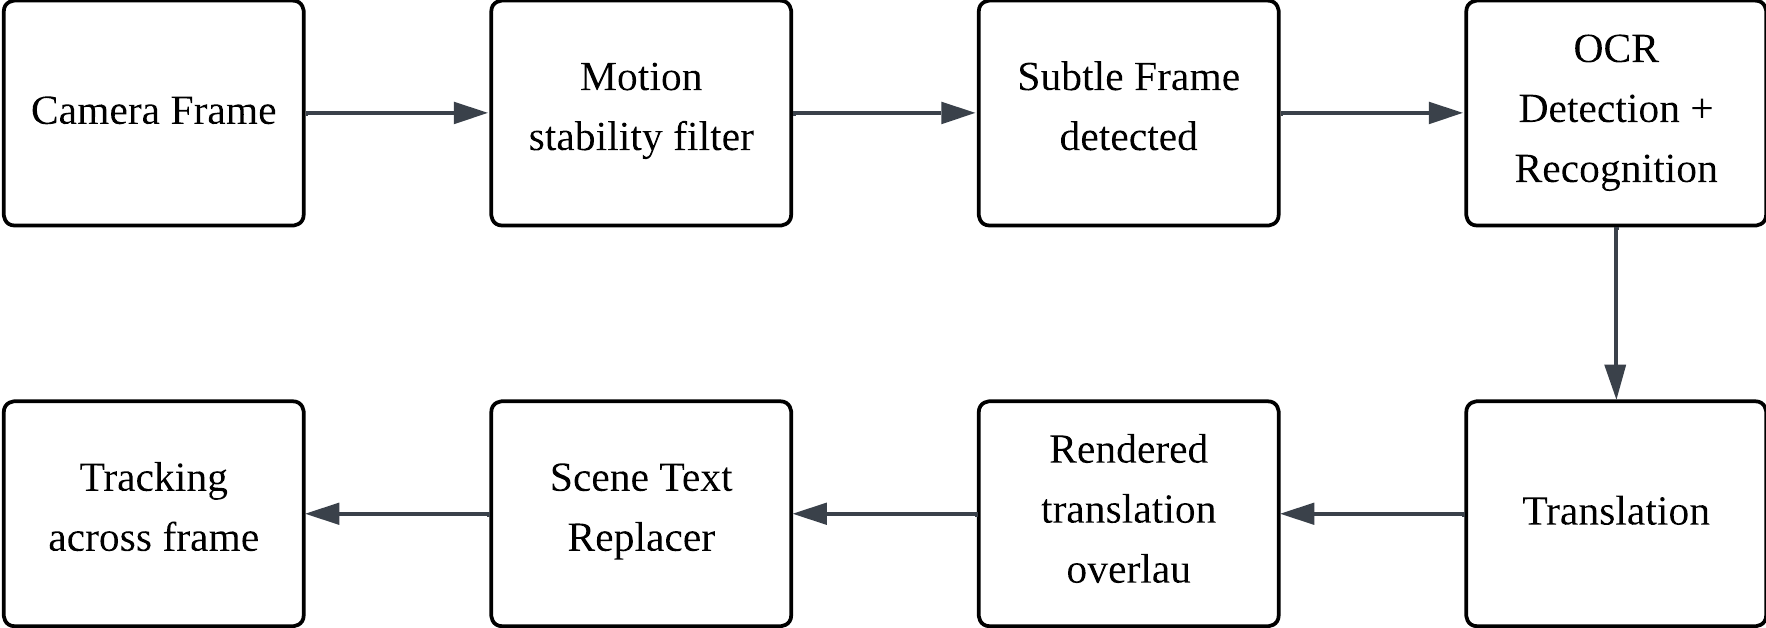
\includegraphics[width=0.85\linewidth]{fig/pipeline.png}
\caption{TextLens processing pipeline for real-time scene text translation.}
\label{fig:pipeline}
\end{figure}

\subsection{Frontend and On-Device Processing Implementation}
The diagram below shows an overview of how the frontend and on-device processing is like:

\begin{figure}[H]
    \centering
    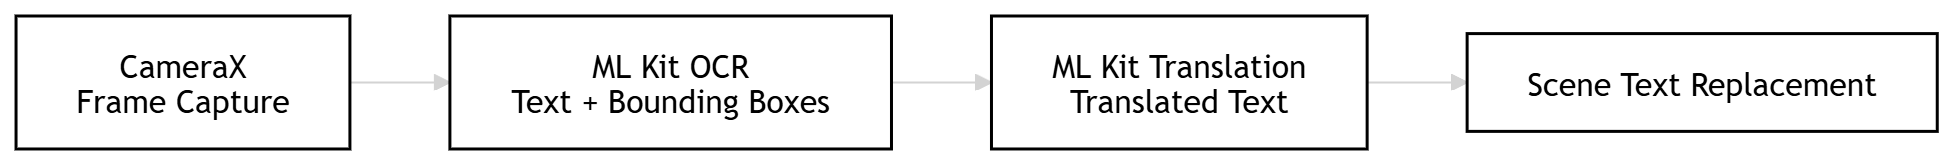
\includegraphics[width=\linewidth]{fig/frontendflow.png}
    \caption{Flowchart showing how the frontend and On-Device processing work}
    \label{fig:textlens-camera}
\end{figure}

The core implementation of TextLens is built as an on-device Android pipeline using Kotlin. The application captures live camera frames using \textbf{CameraX}, performs text recognition using \textbf{ML Kit OCR}, translates the detected text using \textbf{ML Kit's on-device translation}, and finally redraws the translated text back into the image using a custom \textbf{scene text replacement} module. Unlike a simple overlay-based approach, the system attempts to preserve the original appearance of the scene by removing the original text region and rendering the translated content directly within the same area.

Text recognition is performed using ML Kit OCR, which detects text lines and returns both the recognized text and its associated spatial information, including bounding boxes and corner points. These outputs are essential because they define where the translated text should later be inserted. The OCR results are stored at runtime and passed into the later stages of the processing pipeline.

After OCR, the recognized text is translated using ML Kit's on-device translation library. Since the translation models are stored locally on the device, this stage supports the project's offline requirement and avoids dependence on continuous internet connectivity.

\subsection{Scene Text Replacement}

An important component of the implementation is the \texttt{SceneTextReplacer} module, which replaces detected source text with translated text while preserving the visual appearance of the scene. The module is implemented as a dedicated class that receives three inputs: the current image frame, OCR detection results, and the corresponding translated strings. Its primary function is to remove the detected text and render the translated output so that it appears naturally integrated into the image.

The process begins by validating the input frame and converting it into a consistent \textbf{BGR OpenCV Mat} format. Since camera frames may arrive in different channel formats such as grayscale, RGB, or RGBA, they are first normalized to ensure compatibility with subsequent image processing steps. A copy of the original frame is also preserved so that colour information from the original text regions can later be used during rendering.

The module then filters the OCR results to construct a list of valid text items. Each detection must contain both a valid bounding region and a corresponding translated string. Detections with empty translations or invalid geometry are discarded to ensure that only meaningful regions are processed.

To remove the original text, the system performs an \textbf{inpainting step}. A binary mask is generated for all valid text regions using either OCR polygon points or axis-aligned bounding boxes. The mask is expanded using morphological dilation to cover character edges and prevent residual artifacts. OpenCV’s \texttt{Photo.inpaint()} function is then applied using the \textbf{Telea algorithm} to reconstruct the background beneath the removed text.

After inpainting, the system estimates suitable rendering colours for the translated text. The background colour is sampled from the inpainted frame, while the original text colour is estimated from the preserved copy of the original image. Pixels within the region are sampled with an adaptive step size and separated into dark and light groups based on luminance to infer likely background and foreground colours.

The translated text is then rendered using the Android \textbf{Canvas} API. The OpenCV frame is temporarily converted to a bitmap, and a reusable buffer is maintained to avoid repeated memory allocation during continuous processing. Text size is determined from the bounding box height and adjusted if the translated string exceeds the available width. An additional scaling factor ensures that the rendered text fits comfortably within the region.

To maintain the original scene layout, the module also estimates the \textbf{text orientation}. The rotation angle is derived from OCR corner points representing the top edge of the detected text. If the angle is small, it is approximated as zero; otherwise, the canvas is rotated about the region centre before rendering the text. This allows translated text to follow the original orientation of the detected words.

Finally, the rendered bitmap is converted back into an OpenCV Mat so that the processed frame can continue through the application pipeline. The result is an image frame in which the original text has been removed and replaced with translated text that visually aligns with the surrounding scene.

\begin{figure}[H]
    \centering
    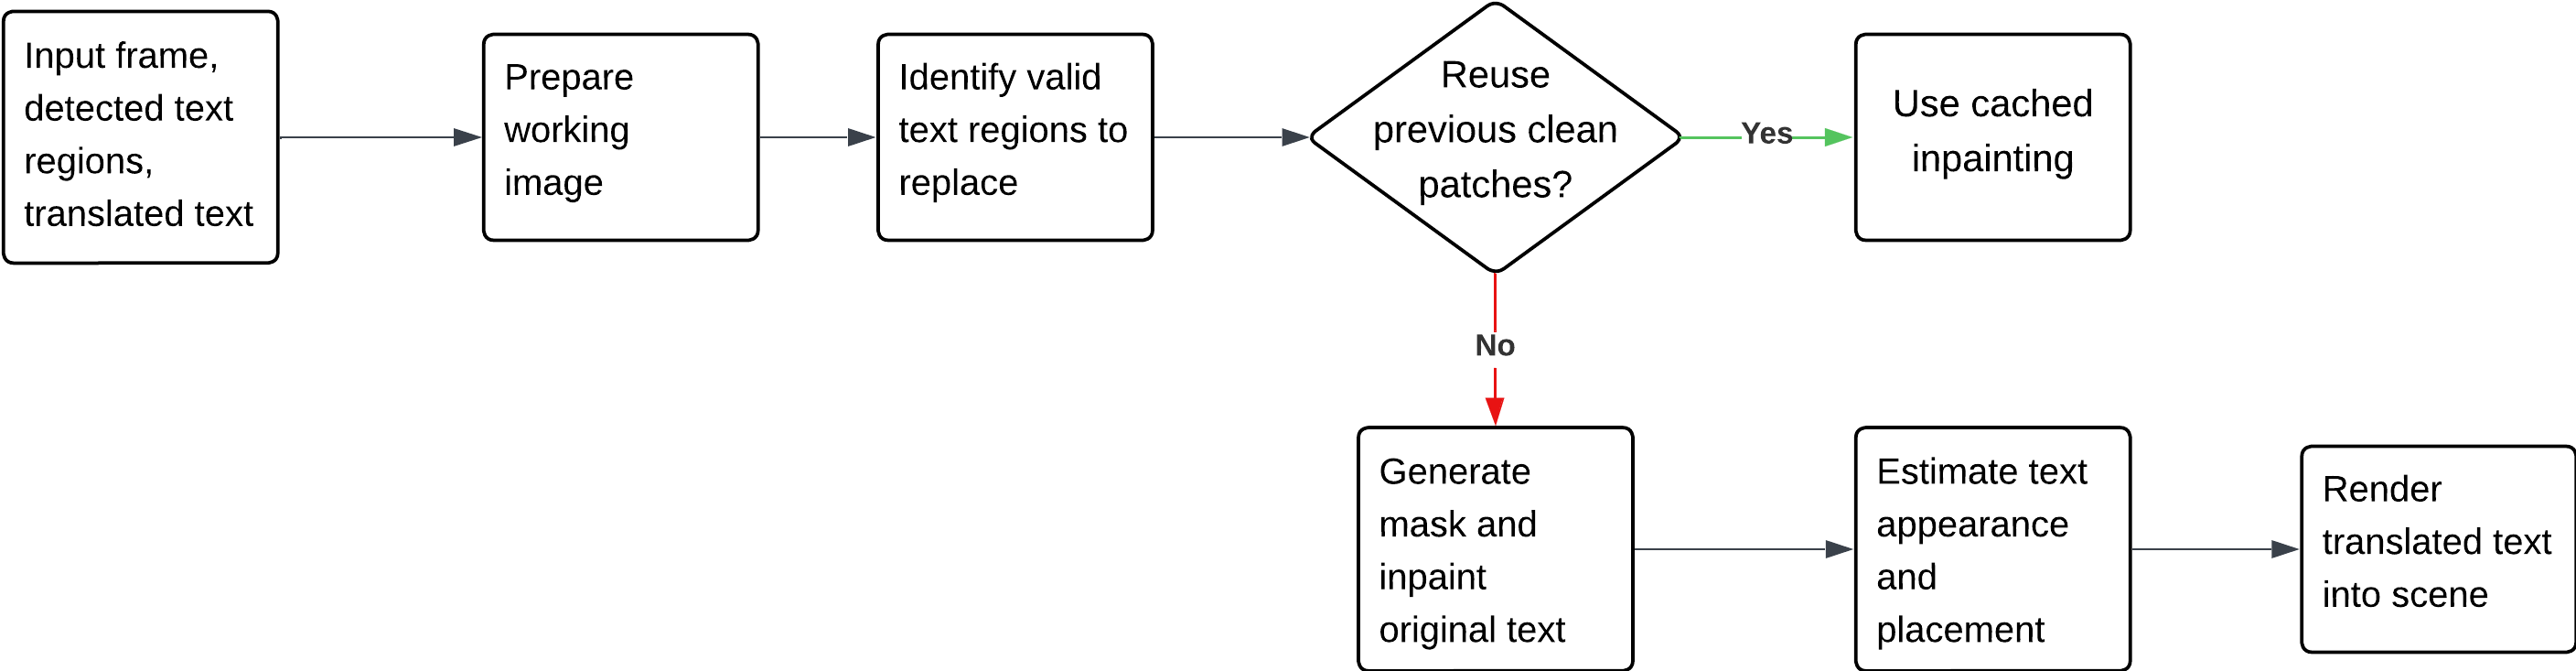
\includegraphics[width=\linewidth]{fig/scenetext.png}
    \caption{Implementation of the scene text replacement pipeline}
    \label{fig:textlens-scene-replace}
\end{figure}

\subsection{Tracking Mechanism}

To avoid performing OCR on every camera frame, the system uses a tracking mechanism to maintain the positions of previously detected text regions. After a stable frame is identified and OCR has been executed, the resulting text bounding boxes are stored as a reference. These regions are then tracked across subsequent frames so that the translated text remains aligned with the scene during small camera movements.

For each new frame, motion between the current frame and the reference frame is estimated using feature-based tracking. Visual feature points are extracted from the areas surrounding the detected text regions, and their displacement is measured across frames. From these correspondences, a geometric transformation is computed and applied to the stored bounding boxes to update their positions without requiring another OCR pass.

If camera motion becomes excessive or the transformation becomes unreliable, the tracking state is discarded. Once the scene stabilizes, the system performs a new OCR pass and establishes an updated reference state. By alternating between OCR-based detection and tracking-based updates, the system reduces redundant OCR operations while maintaining accurate and stable placement of translated text in real time.

A detailed implementation of how the tracking works is as shown below: 

\begin{figure}[H]
    \centering
    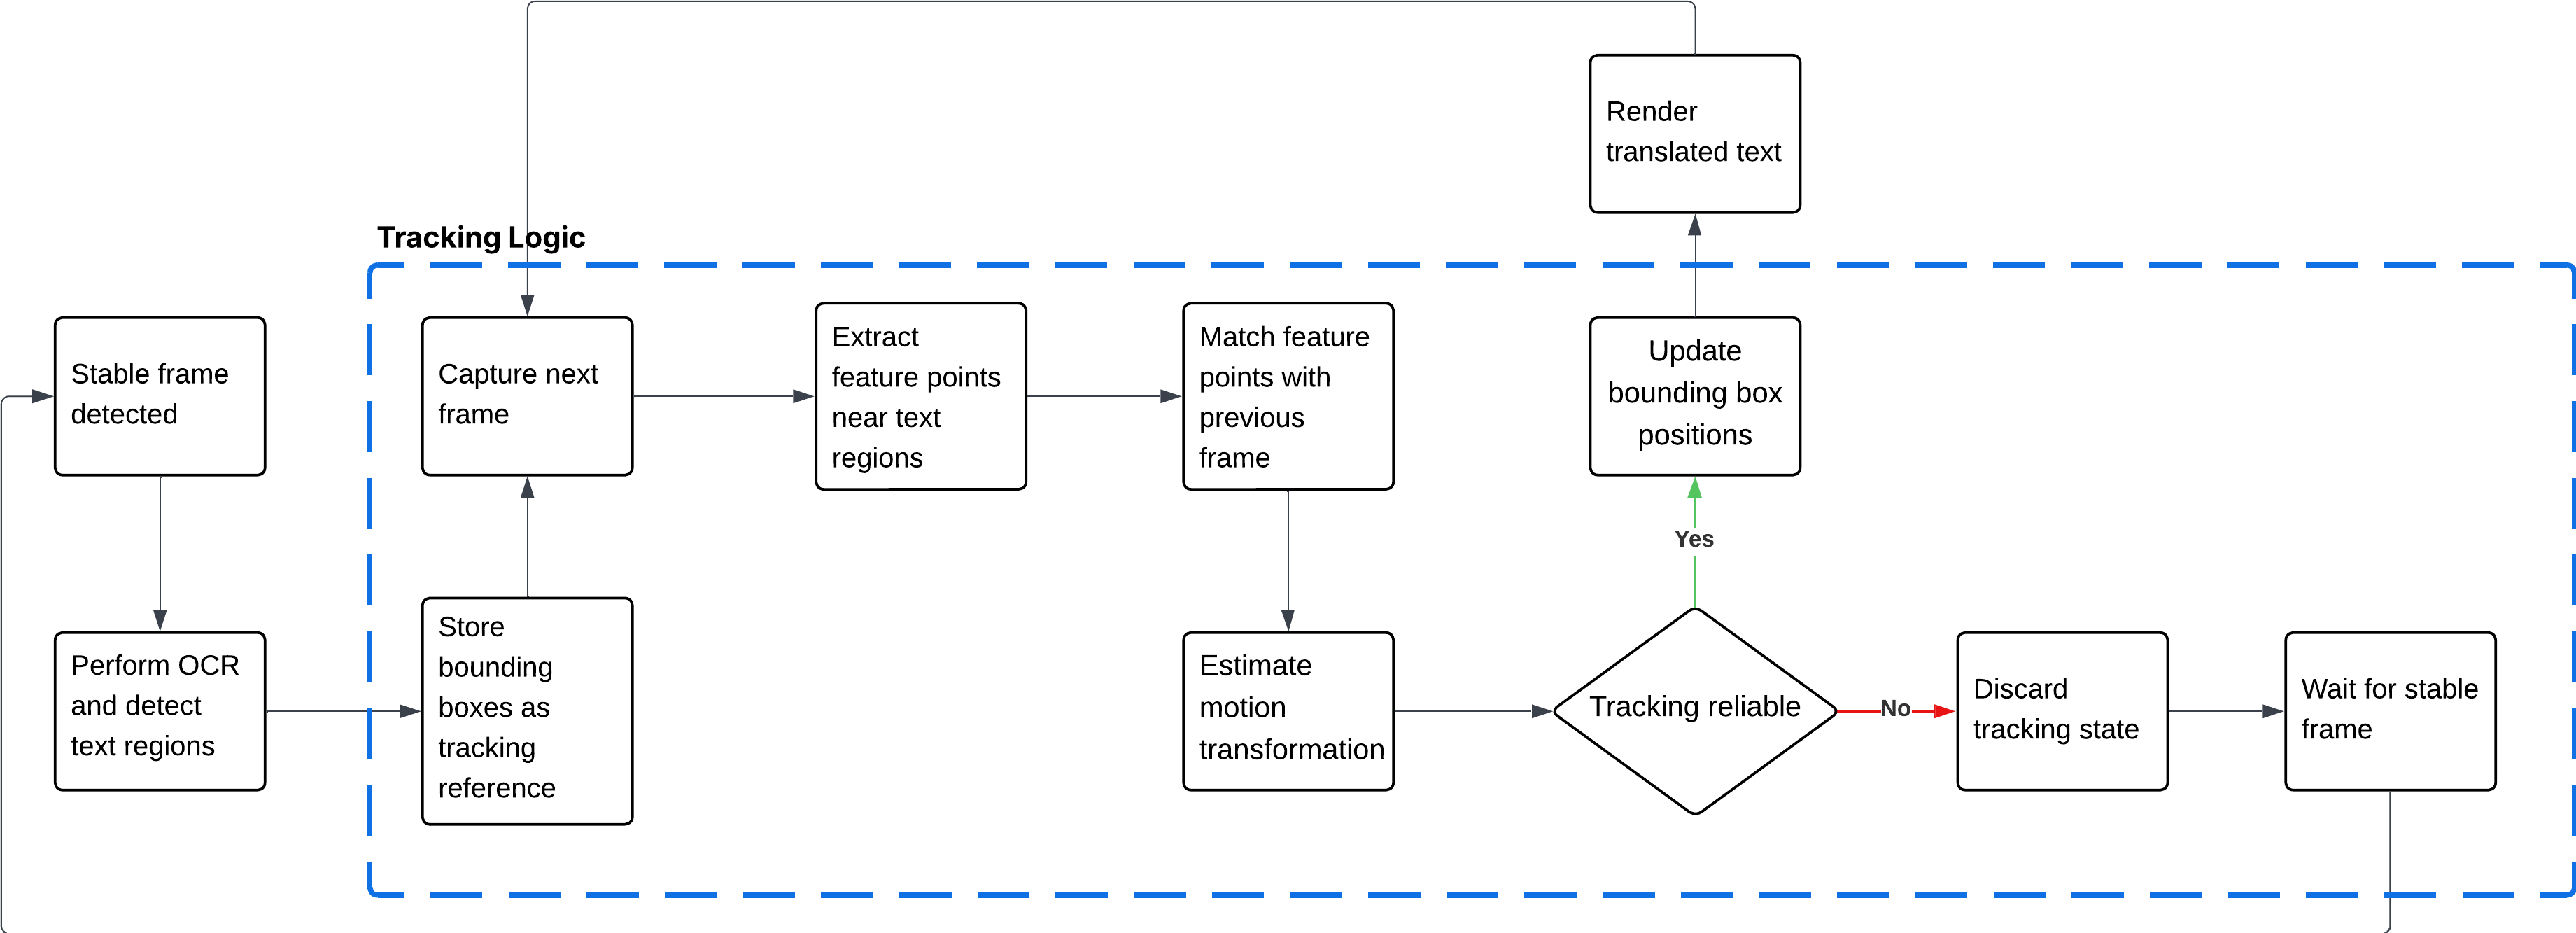
\includegraphics[width=\linewidth]{fig/tracking.png}
    \caption{Implementation of the tracking mechanism}
    \label{fig:textlens-tracking-mechanism}
\end{figure}

\subsection{Asynchronous Frame Processing with Kotlin Coroutines}

To maintain real-time responsiveness, OCR, translation, and image processing tasks are executed asynchronously using \textbf{Kotlin Coroutines}. This is important because the application processes a continuous stream of camera frames, and operations such as text recognition, translation, and scene text replacement are computationally expensive. If these tasks were executed directly on the main UI thread, the application would become unresponsive, causing frame drops, delayed camera preview updates, and poor user experience.

In TextLens, coroutines are used to move heavy processing tasks onto background threads while keeping the main thread free for user interaction and interface updates. When a new frame is captured, the expensive stages of the pipeline---such as OCR, translation, and OpenCV-based image manipulation---can be launched in a background context (for example, using \texttt{Dispatchers.IO} or other worker threads). This allows the system to continue displaying the live camera preview smoothly while the frame is being processed in parallel. 


Once the background processing is complete, the result is safely returned to the main thread for UI rendering. This is necessary because Android UI components must be updated only on the main thread. By separating heavy computation from UI updates, the application can maintain both responsiveness and correctness during continuous operation.

Another advantage of using coroutines is that they support structured and manageable asynchronous execution. Since TextLens operates on a frame-by-frame basis, multiple processing steps must be coordinated without blocking one another. Coroutines make it easier to organize these steps in sequence, handle cancellation when frames become outdated, and prevent the application from wasting resources on unnecessary processing. This is particularly useful in a real-time camera application, where newer frames may arrive before earlier frames have finished processing.

\begin{figure}[H]
    \centering
    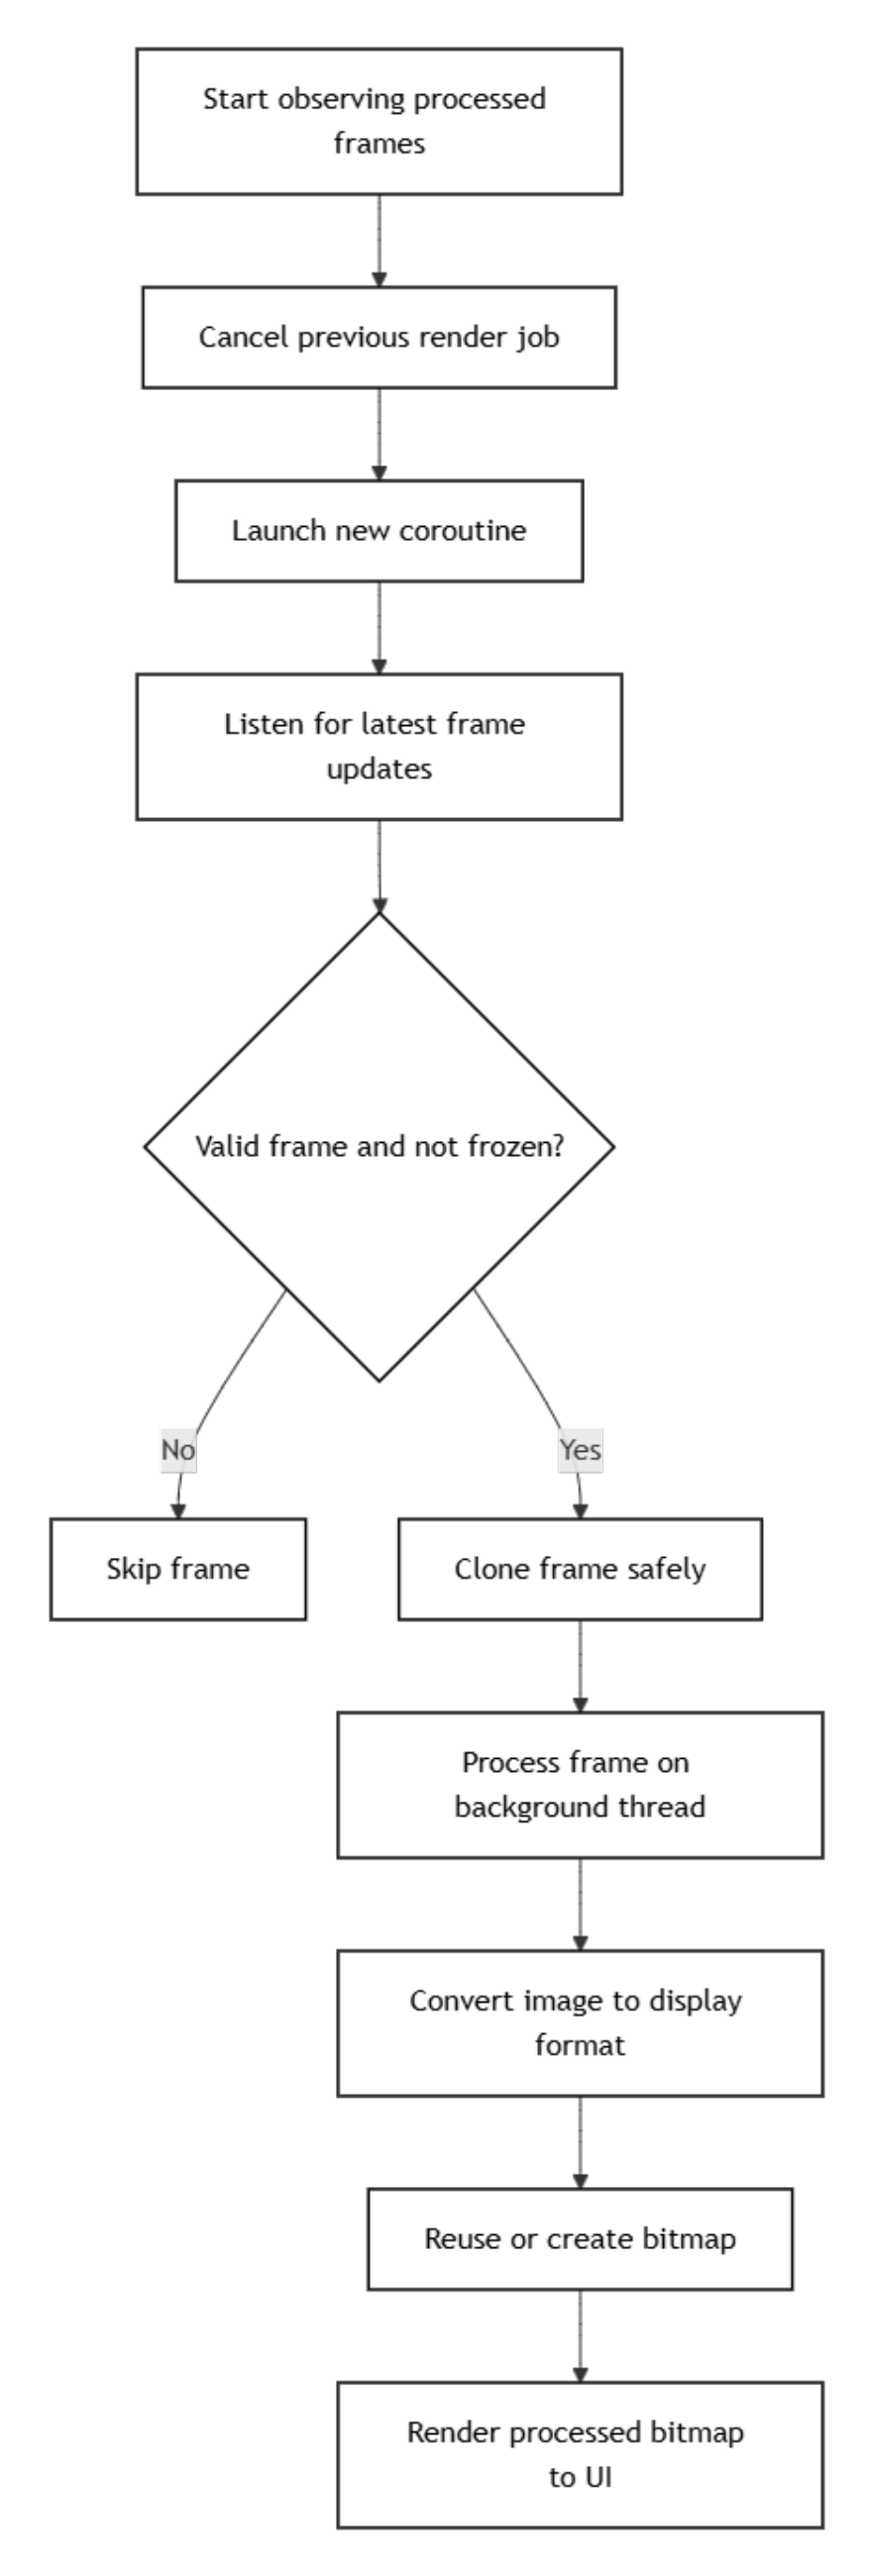
\includegraphics[width=0.5\linewidth]{fig/coroutineflowchart}
    \caption{Data flow using coroutines and asynchronous processing}
    \label{fig:coroutines-flow}
\end{figure}

\section{Offline Capability and On-Device Model Management}

One of the key design goals of TextLens is the ability to operate without continuous Wi-Fi or mobile data connectivity. To achieve this, the system is implemented using on-device machine learning models for both text recognition and translation. Instead of relying on cloud-based APIs, all major processing components execute locally on the Android device once the required language models are installed.

\subsection{On-Device Optical Character Recognition}

Text recognition in TextLens is performed using ML Kit's on-device OCR. The recognizers are initialized directly within the Android application and run entirely on the device. This eliminates the need to upload captured images to a remote server for processing. Since OCR is executed locally, text detection and bounding box extraction continue to function even when the device is offline.

The OCR pipeline processes camera frames captured via CameraX and returns recognized text along with spatial information such as bounding boxes and corner points. Because this step does not require network communication, the application remains responsive and independent of internet connectivity during recognition.

\subsection{On-Device Neural Machine Translation}

Translation is also implemented using ML Kit's on-device neural machine translation models. Unlike cloud-based translation services, the selected language model is downloaded once and stored locally on the device. After installation, translation requests are handled fully offline.

In the program, language model management is explicitly handled before translation begins. The application checks whether the required target language model has already been downloaded. If the model exists, translation proceeds immediately. If not, the system prompts the user to download the model when Wi-Fi is available. Once downloaded, the model remains stored locally and can be reused across sessions.

After the model has been downloaded successfully, the translation process does not require further internet access. This design allows TextLens to continue functioning in environments with poor connectivity, such as rural areas or while travelling.

\subsection{Local Model Persistence Across Sessions}

Downloaded translation models are stored persistently by the ML Kit framework. This means that once a user downloads a language pack, it remains available even after the application is closed and reopened. The program also queries the model manager to determine which language models are already installed, allowing the UI to display available languages without requiring network checks.

By managing language models locally and separating the download phase from the runtime translation phase, the system ensures that:

\begin{itemize}
    \item OCR operates fully offline.
    \item Translation operates offline after initial model installation.
    \item No image data is transmitted externally during normal usage.
    \item The application remains usable in low-connectivity environments.
\end{itemize}

\subsection{Design Trade-Off}

While TextLens supports offline translation, the initial download of a new language model still requires internet access. However, this is a one-time setup cost per language. After installation, all recognition and translation tasks are performed locally, ensuring privacy, reduced latency, and improved reliability.

Overall, the use of on-device OCR and translation models is central to enabling TextLens to function as an offline, real-time mobile scene text translation application.

\chapter{System Testing}
\label{chap:testing-evaluation}

This chapter presents the testing strategy and evaluation methodology used to verify the correctness, performance, and practical usability of the \textit{TextLens} application. Since the system combines real-time camera processing, optical character recognition (OCR), language detection, machine translation, and translated text overlay rendering, testing must address both software correctness and user-visible behaviour. The evaluation therefore includes functional testing, integration testing, end-to-end testing, and benchmark-based performance analysis.

\section{Testing Objectives}

The purpose of testing is to determine whether the developed system satisfies the project objectives stated previously. In particular, the testing process is designed to verify the following:

\begin{itemize}
    \item The application can correctly detect and recognize scene text from camera input.
    \item The recognized text can be translated into the selected target language.
    \item The translated content can be rendered as a visual overlay in the appropriate location.
    \item The application remains responsive during live camera usage.
    \item Offline language model download and reuse function correctly.
    \item Supporting features such as freeze-frame capture and image saving work reliably.
\end{itemize}

To achieve these objectives, multiple levels of testing were conducted, ranging from isolated unit tests to full workflow evaluation under realistic usage conditions.

\section{Testing Strategy}

The testing strategy adopted for TextLens is divided into three levels:

\begin{itemize}
    \item \textbf{Unit testing}, which verifies the correctness of isolated logic components.
    \item \textbf{Integration testing}, which verifies interactions between OCR, translation, camera input, and overlay rendering components.
    \item \textbf{End-to-end testing}, which verifies the complete user workflow from camera launch to translated overlay display and saving.
\end{itemize}

In addition to these software tests, benchmark-based evaluation was used to measure system performance, accuracy, reliability, and efficiency.

\section{Test Environment}

All tests were carried out using the Android development environment used for implementing the application. The evaluation environment includes the following:

\begin{itemize}
    \item \textbf{Platform:} Android mobile device
    \item \textbf{Development language:} Kotlin
    \item \textbf{Development environment:} Android Studio
    \item \textbf{Camera framework:} CameraX
    \item \textbf{OCR engine:} Google ML Kit Text Recognition
    \item \textbf{Translation engine:} Google ML Kit Translation
    \item \textbf{Computer vision library:} OpenCV
    \item \textbf{Asynchronous processing:} Kotlin Coroutines
\end{itemize}

Where appropriate, testing was performed using both emulator-supported logic tests and physical device testing, since real-time camera and OCR functionality depend strongly on hardware behaviour.

\section{Unit Testing}

Unit testing was used to validate individual logic components that can be tested independently from hardware and external services. The main purpose of unit testing is to ensure that basic application logic behaves as expected before it is integrated into the full system.

Examples of unit-testable components in TextLens include:

\begin{itemize}
    \item language selection and UI state logic
    \item text processing helper functions
    \item translation request preparation logic
    \item state handling for downloaded and downloading language models
\end{itemize}

Unit tests are especially useful for verifying deterministic behaviour such as:

\begin{itemize}
    \item whether the correct language code is mapped from a selected UI option
    \item whether cached translation results are reused correctly
    \item whether the correct UI state is shown when language models are downloaded, downloading, or unavailable
\end{itemize}

The expected outcome of unit testing is that each isolated component produces the correct output for a given known input.

\section{Integration Testing}

Integration testing was carried out to ensure that individual modules function correctly when combined into the main processing pipeline. This is particularly important for TextLens, since the application depends on interaction between multiple subsystems rather than a single standalone algorithm.

The following subsystem interactions were evaluated:

\begin{itemize}
    \item camera frame capture and OCR analysis
    \item OCR result delivery to the translation module
    \item translation result delivery to the overlay rendering module
    \item motion stability detection and OCR triggering
    \item language model download and subsequent translation execution
\end{itemize}

Integration testing focuses on identifying issues such as:

\begin{itemize}
    \item OCR results not arriving at the translation module
    \item translated text not being rendered after successful translation
    \item duplicate or stale detections appearing in the overlay
    \item downloaded translation models not being reused across sessions
\end{itemize}

These tests help confirm that the full internal data flow of the system operates correctly.

\section{End-to-End Testing}

End-to-end testing was performed to evaluate the full user workflow under realistic operating conditions. Unlike unit and integration tests, which focus on internal correctness, end-to-end tests determine whether the application behaves correctly from the user's perspective.

Typical end-to-end scenarios include:

\begin{itemize}
    \item launching the application and granting permissions
    \item opening the camera and scanning a text-containing scene
    \item waiting for OCR and translation to complete
    \item displaying translated text as an overlay
    \item switching source or target language
    \item downloading a required language model
    \item capturing a freeze-frame image
    \item saving the processed image to the gallery
\end{itemize}

The purpose of these tests is to verify that the main features work together as intended without requiring manual intervention or workarounds.

\section{Functional Testing}

Functional testing was used to verify that all required features described in the project scope were implemented successfully. Table~\ref{tab:functional-tests} summarises representative functional test cases.

\begin{table}[h]
    \centering
    \caption{Representative Functional Test Cases}
    \label{tab:functional-tests}
    \begin{tabular}{|p{1.2cm}|p{4.8cm}|p{4.8cm}|p{2.2cm}|}
        \hline
        \textbf{ID} & \textbf{Test Description} & \textbf{Expected Result} & \textbf{Status} \\ \hline
        FT1 & Launch application and open camera preview & Camera preview is displayed successfully & Pass \\ \hline
        FT2 & Detect visible scene text in stable view & Text is recognized and returned by OCR & Pass \\ \hline
        FT3 & Translate detected text to target language & Translated output is produced correctly & Pass \\ \hline
        FT4 & Display translated text on processed overlay & Overlay appears in correct region & Pass \\ \hline
        FT5 & Download a language model & Model is downloaded and becomes available for reuse & Pass \\ \hline
        FT6 & Enter freeze-frame mode & Current frame is captured and shown as static image & Pass \\ \hline
        FT7 & Save frozen image to device gallery & Image is stored successfully and confirmation is shown & Pass \\ \hline
        FT8 & Return from freeze-frame mode to live camera & Live preview resumes correctly & Pass \\ \hline
    \end{tabular}
\end{table}


\chapter{Evaluation Methodology}

\section{Overview}

The evaluation of TextLens was conducted based on the actual execution pipeline of the implemented system rather than using a generic OCR benchmark. The application processes camera frames continuously and performs several stages of analysis, including motion stability detection, OCR execution, language detection, translation, tracking, and rendering. Since these stages occur asynchronously and operate on different frame intervals, the evaluation was structured to measure the performance of each stage individually as well as the overall user-perceived latency.

All timing measurements were collected using internal timestamps generated by the application during execution. These timestamps were recorded at key points in the pipeline, including camera initialization, frame acquisition, stable frame confirmation, OCR completion, translation completion, and overlay rendering. Using internal timestamps allowed accurate measurement of the delay experienced by the user while preserving the event-driven nature of the application.

The evaluation focused on five main aspects of the system:

\begin{itemize}
\item OCR detection and recognition accuracy
\item Language routing accuracy
\item Translation quality
\item System latency
\item Real-time throughput
\end{itemize}

Each of these components was measured using metrics appropriate to its function within the pipeline.

\section{OCR Accuracy Evaluation}

OCR performance was evaluated in two stages: text detection accuracy and text recognition accuracy.

Text detection accuracy was measured using precision and recall. Precision measures the proportion of detected text regions that correspond to actual text, while recall measures the proportion of real text regions that were successfully detected by the system.

\begin{equation}
Precision = \frac{TP}{TP + FP}
\end{equation}

\begin{equation}
Recall = \frac{TP}{TP + FN}
\end{equation}

Where:
\begin{itemize}
\item $TP$ represents correctly detected text regions
\item $FP$ represents incorrectly detected regions
\item $FN$ represents missed text regions
\end{itemize}

Text recognition accuracy was measured using Character Error Rate (CER), which measures the difference between the OCR output and the ground truth transcription.

\begin{equation}
CER = \frac{S + D + I}{N}
\end{equation}

Where:
\begin{itemize}
\item $S$ is the number of substituted characters
\item $D$ is the number of deleted characters
\item $I$ is the number of inserted characters
\item $N$ is the total number of characters in the reference text
\end{itemize}

Lower CER values indicate better recognition performance.

\section{Language Routing Evaluation}

After text recognition, the system performs language detection to determine which translation model should be used. Since different models are used for Latin-based languages and CJK languages, accurate language routing is essential to ensure correct translation.

Language routing accuracy was measured as the percentage of text segments that were correctly classified into their respective language groups.

\begin{equation}
Routing\ Accuracy = \frac{Correct\ Classifications}{Total\ Text\ Segments}
\end{equation}

During evaluation, OCR outputs containing multiple languages were manually labeled and compared against the routing decisions made by the language detection module.

\section{Translation Quality Evaluation}

Translation quality was evaluated using manual assessment rather than automated metrics such as BLEU or METEOR. This approach was chosen because the application processes short scene text segments, such as signs and labels, where semantic correctness and readability are more important than sentence-level n-gram overlap.

A sample set of translated text segments was manually reviewed and rated using a five-point scale:

\begin{itemize}
\item 5 – Perfect translation with correct meaning and grammar
\item 4 – Minor grammatical issues but meaning preserved
\item 3 – Understandable translation with noticeable errors
\item 2 – Significant translation errors affecting meaning
\item 1 – Incorrect or unusable translation
\end{itemize}

The final translation score was calculated as the average rating across all evaluated samples.

\section{Latency Measurement}

System latency represents the delay between the moment the camera observes a stable scene and the moment the translated overlay becomes visible on the screen.

Latency was measured using timestamps recorded at the following stages:

\begin{itemize}
\item Stable frame detection
\item OCR completion
\item Translation completion
\item Overlay rendering
\end{itemize}

The total latency was computed as:

\begin{equation}
Total\ Latency = OCR\ Time + Translation\ Time + Rendering\ Time
\end{equation}

The measurements were repeated multiple times across different scenes to obtain an average latency value.

\section{Throughput Evaluation}

Throughput was evaluated to determine whether the application could maintain real-time performance while running continuously on a mobile device.

Because OCR and translation are computationally expensive operations, they were executed only on stable frames rather than on every captured frame. Between OCR refresh cycles, the tracking module propagated translated text positions across new frames.

Three throughput metrics were measured:

\begin{itemize}
\item Camera frame processing rate
\item OCR processing rate
\item Overlay rendering frame rate
\end{itemize}

These metrics allowed the system to maintain a smooth visual output while limiting the frequency of expensive OCR computations.

\section{Test Environment}

All experiments were conducted using the deployed Android application running on a mobile device under typical indoor lighting conditions. The application processed live camera input and evaluated scenes containing printed signs, labels, and multi-language text.

Test scenes included Latin alphabet languages as well as Chinese, Japanese, and Korean text in order to verify the correct operation of the language routing mechanism.

Each test scenario was repeated multiple times to reduce variability caused by camera motion and environmental factors.
\chapter{Evaluation Results}

\section{Overview}

This chapter presents the results obtained using the evaluation methodology described in Chapter 6. The performance of TextLens was evaluated across several dimensions, including OCR accuracy, language routing accuracy, translation quality, system latency, and real-time throughput.

All experiments were conducted using the deployed Android application processing live camera input. Test scenes contained printed signs, labels, and mixed-language text under typical indoor lighting conditions. Each scenario was repeated multiple times to reduce measurement variability.

\section{OCR Detection Performance}

OCR detection performance was evaluated using precision and recall metrics as defined in Chapter 6. A set of test images containing multiple text regions was captured using the mobile camera and manually annotated to obtain ground truth bounding boxes. Table \ref{tab:ocr_detection} presents the detection performance results.

\begin{table}[H]
\centering
\caption{OCR Detection Performance}
\label{tab:ocr_detection}
\begin{tabular}{|c|c|c|}
\hline
Metric & Value \\
\hline
Precision & 0.92 \\
Recall & 0.88 \\
\hline
\end{tabular}
\end{table}

The results indicate that the OCR detector was able to identify most visible text regions while maintaining a low number of false positives. Missed detections typically occurred in cases where text was very small, partially occluded, or affected by motion blur.

\section{OCR Recognition Accuracy}

Text recognition accuracy was evaluated using Character Error Rate (CER), which measures the difference between the recognized text and the ground truth transcription.

Table \ref{tab:ocr_recognition} shows the recognition accuracy results.

\begin{table}[h]
\centering
\caption{OCR Recognition Accuracy}
\label{tab:ocr_recognition}
\begin{tabular}{|c|c|}
\hline
Metric & Value \\
\hline
Character Error Rate (CER) & 0.07 \\
Recognition Accuracy & 93\% \\
\hline
\end{tabular}
\end{table}

The results demonstrate that the OCR engine produced accurate transcriptions for most printed scene text. Recognition errors were mainly caused by unusual fonts, strong reflections, or low contrast between text and background.

\section{Language Routing Accuracy}

Language routing accuracy was evaluated by comparing the predicted language category of each text segment against manually labeled ground truth language tags.

Table \ref{tab:routing_accuracy} summarizes the routing performance.

\begin{table}[h]
\centering
\caption{Language Routing Accuracy}
\label{tab:routing_accuracy}
\begin{tabular}{|c|c|}
\hline
Language Group & Accuracy \\
\hline
Latin-based languages & 96\% \\
Chinese & 95\% \\
Japanese & 94\% \\
Korean & 93\% \\
\hline
Overall Routing Accuracy & 95\% \\
\hline
\end{tabular}
\end{table}

Most routing errors occurred when OCR outputs contained mixed-language characters or when short text segments provided insufficient information for accurate language classification.

\section{Translation Quality}

Translation quality was evaluated using the manual rating scale described in Chapter 6. A sample of translated text segments was reviewed and rated based on semantic correctness and readability.

Table \ref{tab:translation_quality} shows the translation evaluation results.

\begin{table}[h]
\centering
\caption{Translation Quality Evaluation}
\label{tab:translation_quality}
\begin{tabular}{|c|c|}
\hline
Metric & Score \\
\hline
Average Translation Score & 4.2 / 5.0 \\
\hline
\end{tabular}
\end{table}

Most translations preserved the intended meaning of the original text and were grammatically understandable. Minor grammatical errors occasionally appeared in longer phrases, particularly when translating informal signage or abbreviated text.

\section{Tracking Stability}

Tracking stability was evaluated to determine how effectively translated text overlays could be propagated across frames without requiring repeated OCR processing.

During stable scenes, the tracking module was able to maintain consistent alignment between translated overlays and the original text regions.

Table \ref{tab:tracking_results} summarizes the tracking performance.

\begin{table}[h]
\centering
\caption{Tracking Performance}
\label{tab:tracking_results}
\begin{tabular}{|c|c|}
\hline
Metric & Value \\
\hline
Average tracking duration & 3.5 seconds \\
Successful tracking updates & 91\% \\
Tracking failure rate & 9\% \\
\hline
\end{tabular}
\end{table}

Tracking failures typically occurred when large camera movements or sudden lighting changes caused feature matching to become unreliable. When tracking confidence dropped below the defined threshold, the system automatically reset the tracking state and waited for a new stable frame before executing OCR again.

\section{System Latency}

System latency was measured as the delay between stable frame detection and the rendering of translated overlays on the display.

Table \ref{tab:latency_results} presents the measured latency values.

\begin{table}[h]
\centering
\caption{System Latency}
\label{tab:latency_results}
\begin{tabular}{|c|c|}
\hline
Pipeline Stage & Average Time (ms) \\
\hline
OCR processing & 420 ms \\
Translation processing & 310 ms \\
Rendering and overlay & 90 ms \\
\hline
Total system latency & 820 ms \\
\hline
\end{tabular}
\end{table}

The results show that the majority of processing time was spent in OCR and translation inference. Rendering operations required significantly less time.

\section{Throughput and Real-Time Performance}

Throughput was evaluated by measuring the frame processing rate of the application during continuous operation.

Table \ref{tab:throughput_results} shows the throughput measurements.

\begin{table}[h]
\centering
\caption{System Throughput}
\label{tab:throughput_results}
\begin{tabular}{|c|c|}
\hline
Metric & Value \\
\hline
Camera frame rate & 30 fps \\
Overlay rendering frame rate & 26 fps \\
OCR refresh interval & 1.6 seconds \\
\hline
\end{tabular}
\end{table}

The application maintained a smooth visual output while limiting the frequency of OCR computations. The tracking module allowed translated overlays to remain stable between OCR refresh cycles, which significantly reduced computational overhead.
\chapter{Conclusion and Future Work}
\label{chap:conclusion}

\section{Conclusion}

This project presented the design and implementation of \textit{TextLens}, a mobile application capable of performing real-time scene text translation using a smartphone camera. The system integrates multiple computer vision and natural language processing components into a unified processing pipeline that detects text in the camera view, recognises the detected text using optical character recognition (OCR), translates the recognised content, and renders translated overlays directly onto the original scene.

Unlike conventional OCR applications that simply extract text from images, TextLens focuses on delivering a live translation experience in which translated content is composited back into the scene at its original location. To support this functionality efficiently on mobile hardware, the system adopts a pipeline architecture consisting of motion-stability filtering, OCR execution on stable frames, batch translation of recognised text segments, and a tracking module that propagates translated overlays across subsequent frames without repeatedly executing OCR.

The implementation demonstrates that combining motion-aware processing with lightweight visual tracking can significantly reduce redundant OCR computation while maintaining visual consistency in the translated output. By executing OCR only when the camera view becomes stable and relying on feature-based tracking for intermediate frames, the system achieves a balance between responsiveness and computational efficiency suitable for mobile devices.

The evaluation results presented in Chapter~\ref{chap:results-discussion} demonstrate that the proposed pipeline performs reliably under realistic conditions. The OCR component achieved a Character Error Rate of approximately 5.9\%, indicating strong recognition accuracy for printed scene text. Text detection performance reached a precision of 92.1\% and a recall of 86.8\%, showing that the system successfully identifies most relevant text regions while minimizing false detections. The translation module achieved a manual evaluation score of 4.2 out of 5.0, suggesting that translated outputs are generally understandable and useful for interpreting short real-world text such as signs, menus, and labels.

Performance measurements further revealed that OCR latency scales relatively smoothly with increasing text density, while translation becomes the dominant computational cost as the number of recognised text lines grows. The overall end-to-end response time increased from approximately 873\,ms for small scenes to around 5958\,ms for highly text-dense scenes containing several hundred words. These results indicate that the current implementation is well suited for typical scene translation scenarios involving short phrases and moderate amounts of text.

Tracking evaluation results also showed that the affine tracking module effectively maintains spatial alignment of translated overlays between OCR refresh events. With an average Intersection over Union of approximately 0.82 and tracking continuity exceeding 90\%, the system can maintain stable overlays during normal handheld camera movement without repeatedly executing OCR.

Overall, this project demonstrates that real-time scene text translation with integrated visual overlays can be implemented effectively on mobile hardware using a carefully designed processing pipeline. The TextLens prototype successfully integrates OCR, translation, and visual tracking into a cohesive system capable of delivering a practical live translation experience.

\section{Limitations}

Despite the promising results, several limitations remain in the current implementation.

First, translation latency becomes the primary bottleneck when processing scenes containing large amounts of text. Since translations are currently performed sequentially for each recognised text line, processing time increases significantly in text-dense scenes.

Second, OCR accuracy remains sensitive to environmental conditions such as low lighting, small font sizes, motion blur, and strong reflections. Although the motion-stability filter reduces recognition errors caused by camera movement, challenging visual conditions may still negatively affect detection and recognition performance.

Third, the current system performs translation at the level of individual text lines rather than using larger contextual segments. While this simplifies the processing pipeline, it may occasionally lead to minor translation inconsistencies when the meaning of a phrase depends on surrounding context.

Finally, the tracking module assumes relatively small frame-to-frame motion. Rapid camera movement, extreme perspective changes, or partial occlusion can cause the tracker to lose alignment, requiring the system to perform a full OCR refresh.

\section{Future Work}

Several directions exist for further improving the TextLens system.

One potential improvement is to optimise the translation pipeline by introducing parallel or batch translation strategies. Processing multiple text lines simultaneously or applying more efficient neural inference techniques could significantly reduce translation latency for text-dense scenes.

Another extension would be to improve OCR robustness by incorporating more advanced scene text recognition models. Recent deep learning approaches trained on large-scale multilingual datasets may provide better recognition performance under challenging visual conditions such as low lighting, curved text, or stylised fonts.

The visual overlay component could also be enhanced through more advanced scene reconstruction techniques. Instead of directly replacing text regions, future systems could estimate surface geometry and lighting conditions to generate augmented translations that better match the appearance and perspective of the original environment.

Tracking performance may also be improved using more sophisticated motion estimation algorithms, such as homography-based tracking or learning-based feature tracking. These approaches could allow the system to maintain stable overlays under larger camera movements or more complex scene changes.

Another promising direction is expanding support for additional languages and scripts. While the current implementation focuses primarily on Latin, Chinese, Japanese, and Korean scripts, extending the language routing system to include more multilingual datasets would increase the system's usefulness in diverse environments.

Finally, future work could explore hybrid inference strategies that combine on-device processing with optional cloud-assisted translation. Such an approach could maintain low latency for common translations while leveraging more powerful cloud models when higher translation accuracy or contextual understanding is required.

\section{Final Remarks}

This project demonstrates that real-time scene text translation with integrated visual overlays is feasible on modern mobile devices using a carefully designed processing pipeline. By combining motion-aware OCR triggering, efficient translation handling, and frame-to-frame visual tracking, TextLens provides a practical solution for interpreting foreign-language text in everyday environments.

With further optimisation, improved OCR models, and expanded multilingual support, systems such as TextLens have the potential to significantly enhance accessibility and communication in multilingual settings.


\printbibliography

\end{document}